\documentclass[12pt]{article}

\usepackage{geometry,calc}
\usepackage{amsmath,amssymb,hyperref}

\def\quiztitle{Graded Problem 8}
\def\quizsubtitle{Math 4B,\qquad Spring 2017,\qquad Dr. Paul}
\pagestyle{empty}

\geometry{body={6.5in, 9in}, left=1in, top=1in}
\input{../../AxesFunction.tex}

\newcommand{\be}{\begin{enumerate}}
\newcommand{\ee}{\end{enumerate}}

\everymath{\displaystyle}

\begin{document}

%\hfill Student Name: \rule{2in}{.1pt}\\

%\hfill Section Time (e.g. 8am): \rule{2in}{.1pt}\\

\begin{center}
{\Huge \quiztitle}
\vskip.1in
{\large \quizsubtitle}
\end{center}

\begin{enumerate}

 \item Two railway cars that are connected with a spring (permanently attached to both cars) with spring constant $k$ and with a damper that exerts opposite forces on the two cars, of magnitude $c(x_1'-x_2')$ proportional to their relative velocity. The two cars are also subject to air resistance forces $c_1x_1'$ and $c_2x_2'$ proportional to their respective velocities. Therefore, the forces acting on the cars are the force of the spring, the damper, and the air resistance, as summarized in the diagram below.

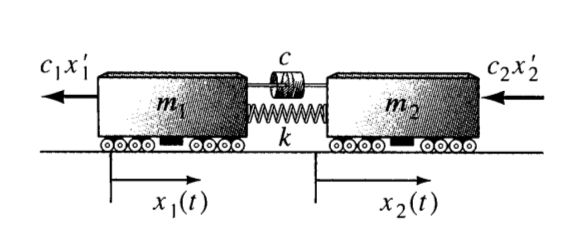
\includegraphics[scale=.5]{railcars}

The positions $x_1,x_2$ of the cars therefore satisfy the system
\begin{align*}
m_1x_1''&=k(x_2-x_1)-c_1x_1'+c(x_2'-x_1')\\
m_2x_2''&=-k(x_2-x_1)-c_2x_2'-c(x_2'-x_1')
\end{align*}

\begin{enumerate}

 \item Convert the second order system to a first order linear system.
 \item Using masses $m_1=m_2=1$, spring constant $k=2$, damping constant $c=1$, and air resistance constants of $c_1=c_2=2$, find the general solution to the linear system.
 \item Using the constants from part (b), determine what happens under the initial conditions in which car 2 starts at rest (that is, $x_2(0)=0$, $x_2'(0)=0$), and car 1 starts at equilibrium position but has initial forward velocity of 2 (that is, $x_1(0)=0$, $x_1'(0)=2$).

\end{enumerate}


\end{enumerate}


\end{document}